% Created by tikzDevice version 0.12.6 on 2025-02-12 05:31:20
% !TEX encoding = UTF-8 Unicode
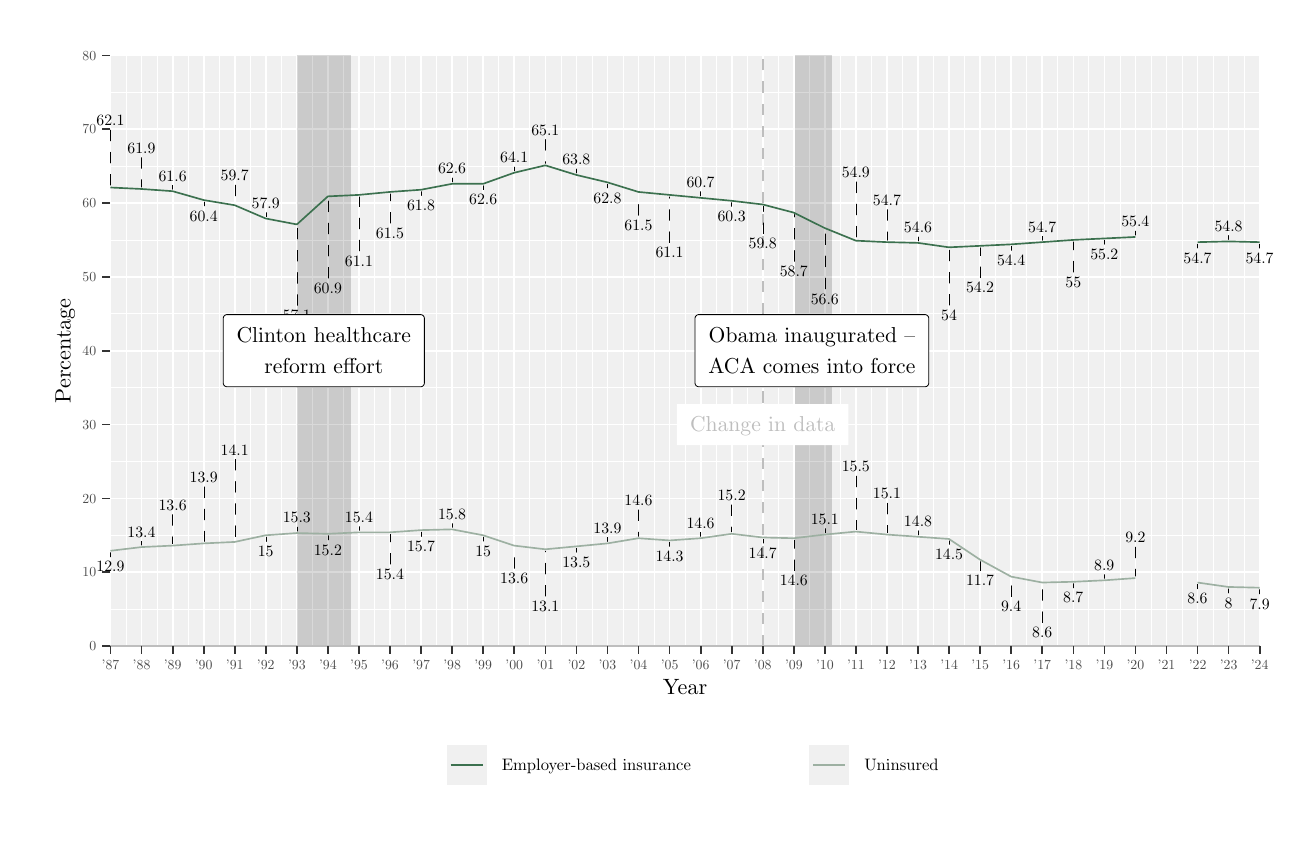
\begin{tikzpicture}[x=1pt,y=1pt]
\definecolor{fillColor}{RGB}{255,255,255}
\path[use as bounding box,fill=fillColor,fill opacity=0.00] (0,0) rectangle (455.30,289.08);
\begin{scope}
\path[clip] (  0.00,  0.00) rectangle (455.30,289.08);
\definecolor{drawColor}{RGB}{255,255,255}
\definecolor{fillColor}{RGB}{255,255,255}

\path[draw=drawColor,line width= 0.6pt,line join=round,line cap=round,fill=fillColor] (  0.00,  0.00) rectangle (455.30,289.08);
\end{scope}
\begin{scope}
\path[clip] (  0.00,  0.00) rectangle (455.30,289.08);
\definecolor{fillColor}{gray}{0.94}

\path[fill=fillColor] ( 29.76, 65.63) rectangle (445.30,279.08);
\definecolor{drawColor}{RGB}{255,255,255}

\path[draw=drawColor,line width= 0.3pt,line join=round] ( 29.76, 78.97) --
	(445.30, 78.97);

\path[draw=drawColor,line width= 0.3pt,line join=round] ( 29.76,105.66) --
	(445.30,105.66);

\path[draw=drawColor,line width= 0.3pt,line join=round] ( 29.76,132.34) --
	(445.30,132.34);

\path[draw=drawColor,line width= 0.3pt,line join=round] ( 29.76,159.02) --
	(445.30,159.02);

\path[draw=drawColor,line width= 0.3pt,line join=round] ( 29.76,185.70) --
	(445.30,185.70);

\path[draw=drawColor,line width= 0.3pt,line join=round] ( 29.76,212.38) --
	(445.30,212.38);

\path[draw=drawColor,line width= 0.3pt,line join=round] ( 29.76,239.06) --
	(445.30,239.06);

\path[draw=drawColor,line width= 0.3pt,line join=round] ( 29.76,265.74) --
	(445.30,265.74);

\path[draw=drawColor,line width= 0.3pt,line join=round] ( 35.56, 65.63) --
	( 35.56,279.08);

\path[draw=drawColor,line width= 0.3pt,line join=round] ( 46.79, 65.63) --
	( 46.79,279.08);

\path[draw=drawColor,line width= 0.3pt,line join=round] ( 58.02, 65.63) --
	( 58.02,279.08);

\path[draw=drawColor,line width= 0.3pt,line join=round] ( 69.23, 65.63) --
	( 69.23,279.08);

\path[draw=drawColor,line width= 0.3pt,line join=round] ( 80.45, 65.63) --
	( 80.45,279.08);

\path[draw=drawColor,line width= 0.3pt,line join=round] ( 91.68, 65.63) --
	( 91.68,279.08);

\path[draw=drawColor,line width= 0.3pt,line join=round] (102.91, 65.63) --
	(102.91,279.08);

\path[draw=drawColor,line width= 0.3pt,line join=round] (114.12, 65.63) --
	(114.12,279.08);

\path[draw=drawColor,line width= 0.3pt,line join=round] (125.34, 65.63) --
	(125.34,279.08);

\path[draw=drawColor,line width= 0.3pt,line join=round] (136.57, 65.63) --
	(136.57,279.08);

\path[draw=drawColor,line width= 0.3pt,line join=round] (147.80, 65.63) --
	(147.80,279.08);

\path[draw=drawColor,line width= 0.3pt,line join=round] (159.01, 65.63) --
	(159.01,279.08);

\path[draw=drawColor,line width= 0.3pt,line join=round] (170.23, 65.63) --
	(170.23,279.08);

\path[draw=drawColor,line width= 0.3pt,line join=round] (181.46, 65.63) --
	(181.46,279.08);

\path[draw=drawColor,line width= 0.3pt,line join=round] (192.69, 65.63) --
	(192.69,279.08);

\path[draw=drawColor,line width= 0.3pt,line join=round] (203.90, 65.63) --
	(203.90,279.08);

\path[draw=drawColor,line width= 0.3pt,line join=round] (215.12, 65.63) --
	(215.12,279.08);

\path[draw=drawColor,line width= 0.3pt,line join=round] (226.35, 65.63) --
	(226.35,279.08);

\path[draw=drawColor,line width= 0.3pt,line join=round] (237.58, 65.63) --
	(237.58,279.08);

\path[draw=drawColor,line width= 0.3pt,line join=round] (248.79, 65.63) --
	(248.79,279.08);

\path[draw=drawColor,line width= 0.3pt,line join=round] (260.01, 65.63) --
	(260.01,279.08);

\path[draw=drawColor,line width= 0.3pt,line join=round] (271.24, 65.63) --
	(271.24,279.08);

\path[draw=drawColor,line width= 0.3pt,line join=round] (282.47, 65.63) --
	(282.47,279.08);

\path[draw=drawColor,line width= 0.3pt,line join=round] (293.68, 65.63) --
	(293.68,279.08);

\path[draw=drawColor,line width= 0.3pt,line join=round] (304.90, 65.63) --
	(304.90,279.08);

\path[draw=drawColor,line width= 0.3pt,line join=round] (316.13, 65.63) --
	(316.13,279.08);

\path[draw=drawColor,line width= 0.3pt,line join=round] (327.36, 65.63) --
	(327.36,279.08);

\path[draw=drawColor,line width= 0.3pt,line join=round] (338.57, 65.63) --
	(338.57,279.08);

\path[draw=drawColor,line width= 0.3pt,line join=round] (349.79, 65.63) --
	(349.79,279.08);

\path[draw=drawColor,line width= 0.3pt,line join=round] (361.02, 65.63) --
	(361.02,279.08);

\path[draw=drawColor,line width= 0.3pt,line join=round] (372.25, 65.63) --
	(372.25,279.08);

\path[draw=drawColor,line width= 0.3pt,line join=round] (383.47, 65.63) --
	(383.47,279.08);

\path[draw=drawColor,line width= 0.3pt,line join=round] (394.68, 65.63) --
	(394.68,279.08);

\path[draw=drawColor,line width= 0.3pt,line join=round] (405.91, 65.63) --
	(405.91,279.08);

\path[draw=drawColor,line width= 0.3pt,line join=round] (417.14, 65.63) --
	(417.14,279.08);

\path[draw=drawColor,line width= 0.3pt,line join=round] (428.36, 65.63) --
	(428.36,279.08);

\path[draw=drawColor,line width= 0.3pt,line join=round] (439.57, 65.63) --
	(439.57,279.08);

\path[draw=drawColor,line width= 0.6pt,line join=round] ( 29.76, 65.63) --
	(445.30, 65.63);

\path[draw=drawColor,line width= 0.6pt,line join=round] ( 29.76, 92.32) --
	(445.30, 92.32);

\path[draw=drawColor,line width= 0.6pt,line join=round] ( 29.76,119.00) --
	(445.30,119.00);

\path[draw=drawColor,line width= 0.6pt,line join=round] ( 29.76,145.68) --
	(445.30,145.68);

\path[draw=drawColor,line width= 0.6pt,line join=round] ( 29.76,172.36) --
	(445.30,172.36);

\path[draw=drawColor,line width= 0.6pt,line join=round] ( 29.76,199.04) --
	(445.30,199.04);

\path[draw=drawColor,line width= 0.6pt,line join=round] ( 29.76,225.72) --
	(445.30,225.72);

\path[draw=drawColor,line width= 0.6pt,line join=round] ( 29.76,252.40) --
	(445.30,252.40);

\path[draw=drawColor,line width= 0.6pt,line join=round] ( 29.76,279.08) --
	(445.30,279.08);

\path[draw=drawColor,line width= 0.6pt,line join=round] ( 29.95, 65.63) --
	( 29.95,279.08);

\path[draw=drawColor,line width= 0.6pt,line join=round] ( 41.16, 65.63) --
	( 41.16,279.08);

\path[draw=drawColor,line width= 0.6pt,line join=round] ( 52.41, 65.63) --
	( 52.41,279.08);

\path[draw=drawColor,line width= 0.6pt,line join=round] ( 63.62, 65.63) --
	( 63.62,279.08);

\path[draw=drawColor,line width= 0.6pt,line join=round] ( 74.84, 65.63) --
	( 74.84,279.08);

\path[draw=drawColor,line width= 0.6pt,line join=round] ( 86.05, 65.63) --
	( 86.05,279.08);

\path[draw=drawColor,line width= 0.6pt,line join=round] ( 97.30, 65.63) --
	( 97.30,279.08);

\path[draw=drawColor,line width= 0.6pt,line join=round] (108.51, 65.63) --
	(108.51,279.08);

\path[draw=drawColor,line width= 0.6pt,line join=round] (119.73, 65.63) --
	(119.73,279.08);

\path[draw=drawColor,line width= 0.6pt,line join=round] (130.94, 65.63) --
	(130.94,279.08);

\path[draw=drawColor,line width= 0.6pt,line join=round] (142.19, 65.63) --
	(142.19,279.08);

\path[draw=drawColor,line width= 0.6pt,line join=round] (153.40, 65.63) --
	(153.40,279.08);

\path[draw=drawColor,line width= 0.6pt,line join=round] (164.62, 65.63) --
	(164.62,279.08);

\path[draw=drawColor,line width= 0.6pt,line join=round] (175.83, 65.63) --
	(175.83,279.08);

\path[draw=drawColor,line width= 0.6pt,line join=round] (187.08, 65.63) --
	(187.08,279.08);

\path[draw=drawColor,line width= 0.6pt,line join=round] (198.30, 65.63) --
	(198.30,279.08);

\path[draw=drawColor,line width= 0.6pt,line join=round] (209.51, 65.63) --
	(209.51,279.08);

\path[draw=drawColor,line width= 0.6pt,line join=round] (220.73, 65.63) --
	(220.73,279.08);

\path[draw=drawColor,line width= 0.6pt,line join=round] (231.97, 65.63) --
	(231.97,279.08);

\path[draw=drawColor,line width= 0.6pt,line join=round] (243.19, 65.63) --
	(243.19,279.08);

\path[draw=drawColor,line width= 0.6pt,line join=round] (254.40, 65.63) --
	(254.40,279.08);

\path[draw=drawColor,line width= 0.6pt,line join=round] (265.62, 65.63) --
	(265.62,279.08);

\path[draw=drawColor,line width= 0.6pt,line join=round] (276.86, 65.63) --
	(276.86,279.08);

\path[draw=drawColor,line width= 0.6pt,line join=round] (288.08, 65.63) --
	(288.08,279.08);

\path[draw=drawColor,line width= 0.6pt,line join=round] (299.29, 65.63) --
	(299.29,279.08);

\path[draw=drawColor,line width= 0.6pt,line join=round] (310.51, 65.63) --
	(310.51,279.08);

\path[draw=drawColor,line width= 0.6pt,line join=round] (321.75, 65.63) --
	(321.75,279.08);

\path[draw=drawColor,line width= 0.6pt,line join=round] (332.97, 65.63) --
	(332.97,279.08);

\path[draw=drawColor,line width= 0.6pt,line join=round] (344.18, 65.63) --
	(344.18,279.08);

\path[draw=drawColor,line width= 0.6pt,line join=round] (355.40, 65.63) --
	(355.40,279.08);

\path[draw=drawColor,line width= 0.6pt,line join=round] (366.64, 65.63) --
	(366.64,279.08);

\path[draw=drawColor,line width= 0.6pt,line join=round] (377.86, 65.63) --
	(377.86,279.08);

\path[draw=drawColor,line width= 0.6pt,line join=round] (389.07, 65.63) --
	(389.07,279.08);

\path[draw=drawColor,line width= 0.6pt,line join=round] (400.29, 65.63) --
	(400.29,279.08);

\path[draw=drawColor,line width= 0.6pt,line join=round] (411.53, 65.63) --
	(411.53,279.08);

\path[draw=drawColor,line width= 0.6pt,line join=round] (422.75, 65.63) --
	(422.75,279.08);

\path[draw=drawColor,line width= 0.6pt,line join=round] (433.96, 65.63) --
	(433.96,279.08);

\path[draw=drawColor,line width= 0.6pt,line join=round] (445.18, 65.63) --
	(445.18,279.08);
\definecolor{fillColor}{RGB}{190,190,190}

\path[fill=fillColor,fill opacity=0.01] ( 97.30, 65.63) rectangle (116.75,279.08);

\path[fill=fillColor,fill opacity=0.01] ( 97.30, 65.63) rectangle (116.75,279.08);

\path[fill=fillColor,fill opacity=0.01] ( 97.30, 65.63) rectangle (116.75,279.08);

\path[fill=fillColor,fill opacity=0.01] ( 97.30, 65.63) rectangle (116.75,279.08);

\path[fill=fillColor,fill opacity=0.01] ( 97.30, 65.63) rectangle (116.75,279.08);

\path[fill=fillColor,fill opacity=0.01] ( 97.30, 65.63) rectangle (116.75,279.08);

\path[fill=fillColor,fill opacity=0.01] ( 97.30, 65.63) rectangle (116.75,279.08);

\path[fill=fillColor,fill opacity=0.01] ( 97.30, 65.63) rectangle (116.75,279.08);

\path[fill=fillColor,fill opacity=0.01] ( 97.30, 65.63) rectangle (116.75,279.08);

\path[fill=fillColor,fill opacity=0.01] ( 97.30, 65.63) rectangle (116.75,279.08);

\path[fill=fillColor,fill opacity=0.01] ( 97.30, 65.63) rectangle (116.75,279.08);

\path[fill=fillColor,fill opacity=0.01] ( 97.30, 65.63) rectangle (116.75,279.08);

\path[fill=fillColor,fill opacity=0.01] ( 97.30, 65.63) rectangle (116.75,279.08);

\path[fill=fillColor,fill opacity=0.01] ( 97.30, 65.63) rectangle (116.75,279.08);

\path[fill=fillColor,fill opacity=0.01] ( 97.30, 65.63) rectangle (116.75,279.08);

\path[fill=fillColor,fill opacity=0.01] ( 97.30, 65.63) rectangle (116.75,279.08);

\path[fill=fillColor,fill opacity=0.01] ( 97.30, 65.63) rectangle (116.75,279.08);

\path[fill=fillColor,fill opacity=0.01] ( 97.30, 65.63) rectangle (116.75,279.08);

\path[fill=fillColor,fill opacity=0.01] ( 97.30, 65.63) rectangle (116.75,279.08);

\path[fill=fillColor,fill opacity=0.01] ( 97.30, 65.63) rectangle (116.75,279.08);

\path[fill=fillColor,fill opacity=0.01] ( 97.30, 65.63) rectangle (116.75,279.08);

\path[fill=fillColor,fill opacity=0.01] ( 97.30, 65.63) rectangle (116.75,279.08);

\path[fill=fillColor,fill opacity=0.01] ( 97.30, 65.63) rectangle (116.75,279.08);

\path[fill=fillColor,fill opacity=0.01] ( 97.30, 65.63) rectangle (116.75,279.08);

\path[fill=fillColor,fill opacity=0.01] ( 97.30, 65.63) rectangle (116.75,279.08);

\path[fill=fillColor,fill opacity=0.01] ( 97.30, 65.63) rectangle (116.75,279.08);

\path[fill=fillColor,fill opacity=0.01] ( 97.30, 65.63) rectangle (116.75,279.08);

\path[fill=fillColor,fill opacity=0.01] ( 97.30, 65.63) rectangle (116.75,279.08);

\path[fill=fillColor,fill opacity=0.01] ( 97.30, 65.63) rectangle (116.75,279.08);

\path[fill=fillColor,fill opacity=0.01] ( 97.30, 65.63) rectangle (116.75,279.08);

\path[fill=fillColor,fill opacity=0.01] ( 97.30, 65.63) rectangle (116.75,279.08);

\path[fill=fillColor,fill opacity=0.01] ( 97.30, 65.63) rectangle (116.75,279.08);

\path[fill=fillColor,fill opacity=0.01] ( 97.30, 65.63) rectangle (116.75,279.08);

\path[fill=fillColor,fill opacity=0.01] ( 97.30, 65.63) rectangle (116.75,279.08);

\path[fill=fillColor,fill opacity=0.01] ( 97.30, 65.63) rectangle (116.75,279.08);

\path[fill=fillColor,fill opacity=0.01] ( 97.30, 65.63) rectangle (116.75,279.08);

\path[fill=fillColor,fill opacity=0.01] ( 97.30, 65.63) rectangle (116.75,279.08);

\path[fill=fillColor,fill opacity=0.01] ( 97.30, 65.63) rectangle (116.75,279.08);

\path[fill=fillColor,fill opacity=0.01] (277.45, 65.63) rectangle (290.57,279.08);

\path[fill=fillColor,fill opacity=0.01] (277.45, 65.63) rectangle (290.57,279.08);

\path[fill=fillColor,fill opacity=0.01] (277.45, 65.63) rectangle (290.57,279.08);

\path[fill=fillColor,fill opacity=0.01] (277.45, 65.63) rectangle (290.57,279.08);

\path[fill=fillColor,fill opacity=0.01] (277.45, 65.63) rectangle (290.57,279.08);

\path[fill=fillColor,fill opacity=0.01] (277.45, 65.63) rectangle (290.57,279.08);

\path[fill=fillColor,fill opacity=0.01] (277.45, 65.63) rectangle (290.57,279.08);

\path[fill=fillColor,fill opacity=0.01] (277.45, 65.63) rectangle (290.57,279.08);

\path[fill=fillColor,fill opacity=0.01] (277.45, 65.63) rectangle (290.57,279.08);

\path[fill=fillColor,fill opacity=0.01] (277.45, 65.63) rectangle (290.57,279.08);

\path[fill=fillColor,fill opacity=0.01] (277.45, 65.63) rectangle (290.57,279.08);

\path[fill=fillColor,fill opacity=0.01] (277.45, 65.63) rectangle (290.57,279.08);

\path[fill=fillColor,fill opacity=0.01] (277.45, 65.63) rectangle (290.57,279.08);

\path[fill=fillColor,fill opacity=0.01] (277.45, 65.63) rectangle (290.57,279.08);

\path[fill=fillColor,fill opacity=0.01] (277.45, 65.63) rectangle (290.57,279.08);

\path[fill=fillColor,fill opacity=0.01] (277.45, 65.63) rectangle (290.57,279.08);

\path[fill=fillColor,fill opacity=0.01] (277.45, 65.63) rectangle (290.57,279.08);

\path[fill=fillColor,fill opacity=0.01] (277.45, 65.63) rectangle (290.57,279.08);

\path[fill=fillColor,fill opacity=0.01] (277.45, 65.63) rectangle (290.57,279.08);

\path[fill=fillColor,fill opacity=0.01] (277.45, 65.63) rectangle (290.57,279.08);

\path[fill=fillColor,fill opacity=0.01] (277.45, 65.63) rectangle (290.57,279.08);

\path[fill=fillColor,fill opacity=0.01] (277.45, 65.63) rectangle (290.57,279.08);

\path[fill=fillColor,fill opacity=0.01] (277.45, 65.63) rectangle (290.57,279.08);

\path[fill=fillColor,fill opacity=0.01] (277.45, 65.63) rectangle (290.57,279.08);

\path[fill=fillColor,fill opacity=0.01] (277.45, 65.63) rectangle (290.57,279.08);

\path[fill=fillColor,fill opacity=0.01] (277.45, 65.63) rectangle (290.57,279.08);

\path[fill=fillColor,fill opacity=0.01] (277.45, 65.63) rectangle (290.57,279.08);

\path[fill=fillColor,fill opacity=0.01] (277.45, 65.63) rectangle (290.57,279.08);

\path[fill=fillColor,fill opacity=0.01] (277.45, 65.63) rectangle (290.57,279.08);

\path[fill=fillColor,fill opacity=0.01] (277.45, 65.63) rectangle (290.57,279.08);

\path[fill=fillColor,fill opacity=0.01] (277.45, 65.63) rectangle (290.57,279.08);

\path[fill=fillColor,fill opacity=0.01] (277.45, 65.63) rectangle (290.57,279.08);

\path[fill=fillColor,fill opacity=0.01] (277.45, 65.63) rectangle (290.57,279.08);

\path[fill=fillColor,fill opacity=0.01] (277.45, 65.63) rectangle (290.57,279.08);

\path[fill=fillColor,fill opacity=0.01] (277.45, 65.63) rectangle (290.57,279.08);

\path[fill=fillColor,fill opacity=0.01] (277.45, 65.63) rectangle (290.57,279.08);

\path[fill=fillColor,fill opacity=0.01] (277.45, 65.63) rectangle (290.57,279.08);

\path[fill=fillColor,fill opacity=0.01] (277.45, 65.63) rectangle (290.57,279.08);
\definecolor{drawColor}{RGB}{190,190,190}

\path[draw=drawColor,line width= 0.6pt,dash pattern=on 4pt off 4pt ,line join=round] (265.59, 65.63) -- (265.59,279.08);

\path[draw=drawColor,line width= 0.6pt,line join=round] ( 29.76, 65.63) -- (445.30, 65.63);
\definecolor{drawColor}{RGB}{60,113,79}

\path[draw=drawColor,line width= 0.6pt,line join=round] ( 29.92,231.32) --
	( 41.13,230.79) --
	( 52.38,229.99) --
	( 63.59,226.79) --
	( 74.81,224.92) --
	( 86.02,220.12) --
	( 97.27,217.98) --
	(108.48,228.12) --
	(119.70,228.65) --
	(130.91,229.72) --
	(142.16,230.52) --
	(153.37,232.66) --
	(164.59,232.66) --
	(175.80,236.66) --
	(187.05,239.33) --
	(198.26,235.86) --
	(209.48,233.19) --
	(220.69,229.72) --
	(231.94,228.65) --
	(243.16,227.59) --
	(254.37,226.52) --
	(265.59,225.19) --
	(276.83,222.25) --
	(288.05,216.65) --
	(299.26,212.11) --
	(310.48,211.58) --
	(321.72,211.31) --
	(332.94,209.71) --
	(344.15,210.24) --
	(355.37,210.78) --
	(366.61,211.58) --
	(377.83,212.38) --
	(389.04,212.91) --
	(400.26,213.45);

\path[draw=drawColor,line width= 0.6pt,line join=round] (422.72,211.58) --
	(433.93,211.84) --
	(445.15,211.58);
\definecolor{drawColor}{RGB}{157,176,162}

\path[draw=drawColor,line width= 0.6pt,line join=round] ( 29.92,100.05) --
	( 41.13,101.39) --
	( 52.38,101.92) --
	( 63.59,102.72) --
	( 74.81,103.25) --
	( 86.02,105.66) --
	( 97.27,106.46) --
	(108.48,106.19) --
	(119.70,106.72) --
	(130.91,106.72) --
	(142.16,107.52) --
	(153.37,107.79) --
	(164.59,105.66) --
	(175.80,101.92) --
	(187.05,100.59) --
	(198.26,101.65) --
	(209.48,102.72) --
	(220.69,104.59) --
	(231.94,103.79) --
	(243.16,104.59) --
	(254.37,106.19) --
	(265.59,104.86) --
	(276.83,104.59) --
	(288.05,105.92) --
	(299.26,106.99) --
	(310.48,105.92) --
	(321.72,105.12) --
	(332.94,104.32) --
	(344.15, 96.85) --
	(355.37, 90.71) --
	(366.61, 88.58) --
	(377.83, 88.85) --
	(389.04, 89.38) --
	(400.26, 90.18);

\path[draw=drawColor,line width= 0.6pt,line join=round] (422.72, 88.58) --
	(433.93, 86.98) --
	(445.15, 86.71);
\definecolor{drawColor}{RGB}{0,0,0}

\path[draw=drawColor,line width= 0.1pt,dash pattern=on 4pt off 4pt ,line join=round,line cap=round] ( 29.92, 97.83) -- ( 29.92, 99.41);

\path[draw=drawColor,line width= 0.1pt,dash pattern=on 4pt off 4pt ,line join=round,line cap=round] ( 41.13,103.52) -- ( 41.13,102.03);

\path[draw=drawColor,line width= 0.1pt,dash pattern=on 4pt off 4pt ,line join=round,line cap=round] ( 52.38,113.17) -- ( 52.38,102.56);

\path[draw=drawColor,line width= 0.1pt,dash pattern=on 4pt off 4pt ,line join=round,line cap=round] ( 63.59,123.18) -- ( 63.59,103.36);

\path[draw=drawColor,line width= 0.1pt,dash pattern=on 4pt off 4pt ,line join=round,line cap=round] ( 74.81,133.14) -- ( 74.81,103.90);

\path[draw=drawColor,line width= 0.1pt,dash pattern=on 4pt off 4pt ,line join=round,line cap=round] ( 86.02,103.36) -- ( 86.02,105.01);

\path[draw=drawColor,line width= 0.1pt,dash pattern=on 4pt off 4pt ,line join=round,line cap=round] ( 97.27,108.64) -- ( 97.27,107.10);

\path[draw=drawColor,line width= 0.1pt,dash pattern=on 4pt off 4pt ,line join=round,line cap=round] (108.48,103.91) -- (108.48,105.55);

\path[draw=drawColor,line width= 0.1pt,dash pattern=on 4pt off 4pt ,line join=round,line cap=round] (119.70,108.85) -- (119.70,107.36);

\path[draw=drawColor,line width= 0.1pt,dash pattern=on 4pt off 4pt ,line join=round,line cap=round] (130.91, 95.19) -- (130.91,106.08);

\path[draw=drawColor,line width= 0.1pt,dash pattern=on 4pt off 4pt ,line join=round,line cap=round] (142.16,105.17) -- (142.16,106.88);

\path[draw=drawColor,line width= 0.1pt,dash pattern=on 4pt off 4pt ,line join=round,line cap=round] (153.37,109.94) -- (153.37,108.43);

\path[draw=drawColor,line width= 0.1pt,dash pattern=on 4pt off 4pt ,line join=round,line cap=round] (164.59,103.51) -- (164.59,105.01);

\path[draw=drawColor,line width= 0.1pt,dash pattern=on 4pt off 4pt ,line join=round,line cap=round] (175.80, 93.64) -- (175.80,101.28);

\path[draw=drawColor,line width= 0.1pt,dash pattern=on 4pt off 4pt ,line join=round,line cap=round] (187.05, 83.60) -- (187.05, 99.95);

\path[draw=drawColor,line width= 0.1pt,dash pattern=on 4pt off 4pt ,line join=round,line cap=round] (198.26, 99.47) -- (198.26,101.01);

\path[draw=drawColor,line width= 0.1pt,dash pattern=on 4pt off 4pt ,line join=round,line cap=round] (209.48,104.96) -- (209.48,103.36);

\path[draw=drawColor,line width= 0.1pt,dash pattern=on 4pt off 4pt ,line join=round,line cap=round] (220.69,114.88) -- (220.69,105.23);

\path[draw=drawColor,line width= 0.1pt,dash pattern=on 4pt off 4pt ,line join=round,line cap=round] (231.94,101.60) -- (231.94,103.15);

\path[draw=drawColor,line width= 0.1pt,dash pattern=on 4pt off 4pt ,line join=round,line cap=round] (243.16,106.73) -- (243.16,105.23);

\path[draw=drawColor,line width= 0.1pt,dash pattern=on 4pt off 4pt ,line join=round,line cap=round] (254.37,116.69) -- (254.37,106.83);

\path[draw=drawColor,line width= 0.1pt,dash pattern=on 4pt off 4pt ,line join=round,line cap=round] (265.59,102.74) -- (265.59,104.21);

\path[draw=drawColor,line width= 0.1pt,dash pattern=on 4pt off 4pt ,line join=round,line cap=round] (276.83, 92.84) -- (276.83,103.95);

\path[draw=drawColor,line width= 0.1pt,dash pattern=on 4pt off 4pt ,line join=round,line cap=round] (288.05,108.11) -- (288.05,106.56);

\path[draw=drawColor,line width= 0.1pt,dash pattern=on 4pt off 4pt ,line join=round,line cap=round] (299.26,127.08) -- (299.26,107.63);

\path[draw=drawColor,line width= 0.1pt,dash pattern=on 4pt off 4pt ,line join=round,line cap=round] (310.48,117.28) -- (310.48,106.56);

\path[draw=drawColor,line width= 0.1pt,dash pattern=on 4pt off 4pt ,line join=round,line cap=round] (321.72,107.34) -- (321.72,105.76);

\path[draw=drawColor,line width= 0.1pt,dash pattern=on 4pt off 4pt ,line join=round,line cap=round] (332.94,102.30) -- (332.94,103.68);

\path[draw=drawColor,line width= 0.1pt,dash pattern=on 4pt off 4pt ,line join=round,line cap=round] (344.15, 92.86) -- (344.15, 96.21);

\path[draw=drawColor,line width= 0.1pt,dash pattern=on 4pt off 4pt ,line join=round,line cap=round] (355.37, 83.46) -- (355.37, 90.07);

\path[draw=drawColor,line width= 0.1pt,dash pattern=on 4pt off 4pt ,line join=round,line cap=round] (366.61, 74.07) -- (366.61, 87.94);

\path[draw=drawColor,line width= 0.1pt,dash pattern=on 4pt off 4pt ,line join=round,line cap=round] (377.83, 86.61) -- (377.83, 88.21);

\path[draw=drawColor,line width= 0.1pt,dash pattern=on 4pt off 4pt ,line join=round,line cap=round] (389.04, 91.47) -- (389.04, 90.02);

\path[draw=drawColor,line width= 0.1pt,dash pattern=on 4pt off 4pt ,line join=round,line cap=round] (400.26,101.45) -- (400.26, 90.82);

\path[draw=drawColor,line width= 0.1pt,dash pattern=on 4pt off 4pt ,line join=round,line cap=round] (422.72, 86.29) -- (422.72, 87.94);

\path[draw=drawColor,line width= 0.1pt,dash pattern=on 4pt off 4pt ,line join=round,line cap=round] (433.93, 84.74) -- (433.93, 86.34);

\path[draw=drawColor,line width= 0.1pt,dash pattern=on 4pt off 4pt ,line join=round,line cap=round] (445.15, 84.42) -- (445.15, 86.07);

\node[text=drawColor,anchor=base,inner sep=0pt, outer sep=0pt, scale=  0.57] at ( 29.92, 92.41) {12.9};

\node[text=drawColor,anchor=base,inner sep=0pt, outer sep=0pt, scale=  0.57] at ( 41.13,105.03) {13.4};

\node[text=drawColor,anchor=base,inner sep=0pt, outer sep=0pt, scale=  0.57] at ( 52.38,114.68) {13.6};

\node[text=drawColor,anchor=base,inner sep=0pt, outer sep=0pt, scale=  0.57] at ( 63.59,124.69) {13.9};

\node[text=drawColor,anchor=base,inner sep=0pt, outer sep=0pt, scale=  0.57] at ( 74.81,134.65) {14.1};

\node[text=drawColor,anchor=base,inner sep=0pt, outer sep=0pt, scale=  0.57] at ( 86.02, 97.93) {15};

\node[text=drawColor,anchor=base,inner sep=0pt, outer sep=0pt, scale=  0.57] at ( 97.27,110.15) {15.3};

\node[text=drawColor,anchor=base,inner sep=0pt, outer sep=0pt, scale=  0.57] at (108.48, 98.48) {15.2};

\node[text=drawColor,anchor=base,inner sep=0pt, outer sep=0pt, scale=  0.57] at (119.70,110.35) {15.4};

\node[text=drawColor,anchor=base,inner sep=0pt, outer sep=0pt, scale=  0.57] at (130.91, 89.77) {15.4};

\node[text=drawColor,anchor=base,inner sep=0pt, outer sep=0pt, scale=  0.57] at (142.16, 99.75) {15.7};

\node[text=drawColor,anchor=base,inner sep=0pt, outer sep=0pt, scale=  0.57] at (153.37,111.45) {15.8};

\node[text=drawColor,anchor=base,inner sep=0pt, outer sep=0pt, scale=  0.57] at (164.59, 98.08) {15};

\node[text=drawColor,anchor=base,inner sep=0pt, outer sep=0pt, scale=  0.57] at (175.80, 88.21) {13.6};

\node[text=drawColor,anchor=base,inner sep=0pt, outer sep=0pt, scale=  0.57] at (187.05, 78.18) {13.1};

\node[text=drawColor,anchor=base,inner sep=0pt, outer sep=0pt, scale=  0.57] at (198.26, 94.04) {13.5};

\node[text=drawColor,anchor=base,inner sep=0pt, outer sep=0pt, scale=  0.57] at (209.48,106.47) {13.9};

\node[text=drawColor,anchor=base,inner sep=0pt, outer sep=0pt, scale=  0.57] at (220.69,116.39) {14.6};

\node[text=drawColor,anchor=base,inner sep=0pt, outer sep=0pt, scale=  0.57] at (231.94, 96.18) {14.3};

\node[text=drawColor,anchor=base,inner sep=0pt, outer sep=0pt, scale=  0.57] at (243.16,108.24) {14.6};

\node[text=drawColor,anchor=base,inner sep=0pt, outer sep=0pt, scale=  0.57] at (254.37,118.20) {15.2};

\node[text=drawColor,anchor=base,inner sep=0pt, outer sep=0pt, scale=  0.57] at (265.59, 97.31) {14.7};

\node[text=drawColor,anchor=base,inner sep=0pt, outer sep=0pt, scale=  0.57] at (276.83, 87.41) {14.6};

\node[text=drawColor,anchor=base,inner sep=0pt, outer sep=0pt, scale=  0.57] at (288.05,109.61) {15.1};

\node[text=drawColor,anchor=base,inner sep=0pt, outer sep=0pt, scale=  0.57] at (299.26,128.58) {15.5};

\node[text=drawColor,anchor=base,inner sep=0pt, outer sep=0pt, scale=  0.57] at (310.48,118.78) {15.1};

\node[text=drawColor,anchor=base,inner sep=0pt, outer sep=0pt, scale=  0.57] at (321.72,108.85) {14.8};

\node[text=drawColor,anchor=base,inner sep=0pt, outer sep=0pt, scale=  0.57] at (332.94, 96.88) {14.5};

\node[text=drawColor,anchor=base,inner sep=0pt, outer sep=0pt, scale=  0.57] at (344.15, 87.43) {11.7};

\node[text=drawColor,anchor=base,inner sep=0pt, outer sep=0pt, scale=  0.57] at (355.37, 78.03) {9.4};

\node[text=drawColor,anchor=base,inner sep=0pt, outer sep=0pt, scale=  0.57] at (366.61, 68.65) {8.6};

\node[text=drawColor,anchor=base,inner sep=0pt, outer sep=0pt, scale=  0.57] at (377.83, 81.19) {8.7};

\node[text=drawColor,anchor=base,inner sep=0pt, outer sep=0pt, scale=  0.57] at (389.04, 92.98) {8.9};

\node[text=drawColor,anchor=base,inner sep=0pt, outer sep=0pt, scale=  0.57] at (400.26,102.95) {9.2};

\node[text=drawColor,anchor=base,inner sep=0pt, outer sep=0pt, scale=  0.57] at (422.72, 80.87) {8.6};

\node[text=drawColor,anchor=base,inner sep=0pt, outer sep=0pt, scale=  0.57] at (433.93, 79.31) {8};

\node[text=drawColor,anchor=base,inner sep=0pt, outer sep=0pt, scale=  0.57] at (445.15, 78.99) {7.9};

\path[draw=drawColor,line width= 0.1pt,dash pattern=on 4pt off 4pt ,line join=round,line cap=round] ( 29.92,252.12) -- ( 29.92,231.96);

\path[draw=drawColor,line width= 0.1pt,dash pattern=on 4pt off 4pt ,line join=round,line cap=round] ( 41.13,242.20) -- ( 41.13,231.43);

\path[draw=drawColor,line width= 0.1pt,dash pattern=on 4pt off 4pt ,line join=round,line cap=round] ( 52.38,232.14) -- ( 52.38,230.63);

\path[draw=drawColor,line width= 0.1pt,dash pattern=on 4pt off 4pt ,line join=round,line cap=round] ( 63.59,224.61) -- ( 63.59,226.14);

\path[draw=drawColor,line width= 0.1pt,dash pattern=on 4pt off 4pt ,line join=round,line cap=round] ( 74.81,232.26) -- ( 74.81,225.56);

\path[draw=drawColor,line width= 0.1pt,dash pattern=on 4pt off 4pt ,line join=round,line cap=round] ( 86.02,222.29) -- ( 86.02,220.76);

\path[draw=drawColor,line width= 0.1pt,dash pattern=on 4pt off 4pt ,line join=round,line cap=round] ( 97.27,188.65) -- ( 97.27,217.34);

\path[draw=drawColor,line width= 0.1pt,dash pattern=on 4pt off 4pt ,line join=round,line cap=round] (108.48,198.51) -- (108.48,227.48);

\path[draw=drawColor,line width= 0.1pt,dash pattern=on 4pt off 4pt ,line join=round,line cap=round] (119.70,208.34) -- (119.70,228.01);

\path[draw=drawColor,line width= 0.1pt,dash pattern=on 4pt off 4pt ,line join=round,line cap=round] (130.91,218.41) -- (130.91,229.08);

\path[draw=drawColor,line width= 0.1pt,dash pattern=on 4pt off 4pt ,line join=round,line cap=round] (142.16,228.39) -- (142.16,229.88);

\path[draw=drawColor,line width= 0.1pt,dash pattern=on 4pt off 4pt ,line join=round,line cap=round] (153.37,234.81) -- (153.37,233.30);

\path[draw=drawColor,line width= 0.1pt,dash pattern=on 4pt off 4pt ,line join=round,line cap=round] (164.59,230.52) -- (164.59,232.01);

\path[draw=drawColor,line width= 0.1pt,dash pattern=on 4pt off 4pt ,line join=round,line cap=round] (175.80,238.72) -- (175.80,237.30);

\path[draw=drawColor,line width= 0.1pt,dash pattern=on 4pt off 4pt ,line join=round,line cap=round] (187.05,248.72) -- (187.05,239.97);

\path[draw=drawColor,line width= 0.1pt,dash pattern=on 4pt off 4pt ,line join=round,line cap=round] (198.26,238.07) -- (198.26,236.50);

\path[draw=drawColor,line width= 0.1pt,dash pattern=on 4pt off 4pt ,line join=round,line cap=round] (209.48,231.12) -- (209.48,232.55);

\path[draw=drawColor,line width= 0.1pt,dash pattern=on 4pt off 4pt ,line join=round,line cap=round] (220.69,221.23) -- (220.69,229.08);

\path[draw=drawColor,line width= 0.1pt,dash pattern=on 4pt off 4pt ,line join=round,line cap=round] (231.94,211.38) -- (231.94,228.01);

\path[draw=drawColor,line width= 0.1pt,dash pattern=on 4pt off 4pt ,line join=round,line cap=round] (243.16,229.88) -- (243.16,228.23);

\path[draw=drawColor,line width= 0.1pt,dash pattern=on 4pt off 4pt ,line join=round,line cap=round] (254.37,224.46) -- (254.37,225.88);

\path[draw=drawColor,line width= 0.1pt,dash pattern=on 4pt off 4pt ,line join=round,line cap=round] (265.59,214.60) -- (265.59,224.54);

\path[draw=drawColor,line width= 0.1pt,dash pattern=on 4pt off 4pt ,line join=round,line cap=round] (276.83,204.60) -- (276.83,221.61);

\path[draw=drawColor,line width= 0.1pt,dash pattern=on 4pt off 4pt ,line join=round,line cap=round] (288.05,194.63) -- (288.05,216.01);

\path[draw=drawColor,line width= 0.1pt,dash pattern=on 4pt off 4pt ,line join=round,line cap=round] (299.26,233.38) -- (299.26,212.75);

\path[draw=drawColor,line width= 0.1pt,dash pattern=on 4pt off 4pt ,line join=round,line cap=round] (310.48,223.36) -- (310.48,212.22);

\path[draw=drawColor,line width= 0.1pt,dash pattern=on 4pt off 4pt ,line join=round,line cap=round] (321.72,213.49) -- (321.72,211.95);

\path[draw=drawColor,line width= 0.1pt,dash pattern=on 4pt off 4pt ,line join=round,line cap=round] (332.94,188.74) -- (332.94,209.07);

\path[draw=drawColor,line width= 0.1pt,dash pattern=on 4pt off 4pt ,line join=round,line cap=round] (344.15,198.67) -- (344.15,209.60);

\path[draw=drawColor,line width= 0.1pt,dash pattern=on 4pt off 4pt ,line join=round,line cap=round] (355.37,208.58) -- (355.37,210.14);

\path[draw=drawColor,line width= 0.1pt,dash pattern=on 4pt off 4pt ,line join=round,line cap=round] (366.61,213.71) -- (366.61,212.22);

\path[draw=drawColor,line width= 0.1pt,dash pattern=on 4pt off 4pt ,line join=round,line cap=round] (377.83,200.72) -- (377.83,211.74);

\path[draw=drawColor,line width= 0.1pt,dash pattern=on 4pt off 4pt ,line join=round,line cap=round] (389.04,210.76) -- (389.04,212.27);

\path[draw=drawColor,line width= 0.1pt,dash pattern=on 4pt off 4pt ,line join=round,line cap=round] (400.26,215.62) -- (400.26,214.09);

\path[draw=drawColor,line width= 0.1pt,dash pattern=on 4pt off 4pt ,line join=round,line cap=round] (422.72,209.40) -- (422.72,210.94);

\path[draw=drawColor,line width= 0.1pt,dash pattern=on 4pt off 4pt ,line join=round,line cap=round] (433.93,214.02) -- (433.93,212.49);

\path[draw=drawColor,line width= 0.1pt,dash pattern=on 4pt off 4pt ,line join=round,line cap=round] (445.15,209.34) -- (445.15,210.94);

\node[text=drawColor,anchor=base,inner sep=0pt, outer sep=0pt, scale=  0.57] at ( 29.92,253.63) {62.1};

\node[text=drawColor,anchor=base,inner sep=0pt, outer sep=0pt, scale=  0.57] at ( 41.13,243.71) {61.9};

\node[text=drawColor,anchor=base,inner sep=0pt, outer sep=0pt, scale=  0.57] at ( 52.38,233.65) {61.6};

\node[text=drawColor,anchor=base,inner sep=0pt, outer sep=0pt, scale=  0.57] at ( 63.59,219.18) {60.4};

\node[text=drawColor,anchor=base,inner sep=0pt, outer sep=0pt, scale=  0.57] at ( 74.81,233.77) {59.7};

\node[text=drawColor,anchor=base,inner sep=0pt, outer sep=0pt, scale=  0.57] at ( 86.02,223.79) {57.9};

\node[text=drawColor,anchor=base,inner sep=0pt, outer sep=0pt, scale=  0.57] at ( 97.27,183.23) {57.1};

\node[text=drawColor,anchor=base,inner sep=0pt, outer sep=0pt, scale=  0.57] at (108.48,193.09) {60.9};

\node[text=drawColor,anchor=base,inner sep=0pt, outer sep=0pt, scale=  0.57] at (119.70,202.91) {61.1};

\node[text=drawColor,anchor=base,inner sep=0pt, outer sep=0pt, scale=  0.57] at (130.91,212.98) {61.5};

\node[text=drawColor,anchor=base,inner sep=0pt, outer sep=0pt, scale=  0.57] at (142.16,222.97) {61.8};

\node[text=drawColor,anchor=base,inner sep=0pt, outer sep=0pt, scale=  0.57] at (153.37,236.32) {62.6};

\node[text=drawColor,anchor=base,inner sep=0pt, outer sep=0pt, scale=  0.57] at (164.59,225.10) {62.6};

\node[text=drawColor,anchor=base,inner sep=0pt, outer sep=0pt, scale=  0.57] at (175.80,240.23) {64.1};

\node[text=drawColor,anchor=base,inner sep=0pt, outer sep=0pt, scale=  0.57] at (187.05,250.23) {65.1};

\node[text=drawColor,anchor=base,inner sep=0pt, outer sep=0pt, scale=  0.57] at (198.26,239.57) {63.8};

\node[text=drawColor,anchor=base,inner sep=0pt, outer sep=0pt, scale=  0.57] at (209.48,225.70) {62.8};

\node[text=drawColor,anchor=base,inner sep=0pt, outer sep=0pt, scale=  0.57] at (220.69,215.81) {61.5};

\node[text=drawColor,anchor=base,inner sep=0pt, outer sep=0pt, scale=  0.57] at (231.94,205.95) {61.1};

\node[text=drawColor,anchor=base,inner sep=0pt, outer sep=0pt, scale=  0.57] at (243.16,231.39) {60.7};

\node[text=drawColor,anchor=base,inner sep=0pt, outer sep=0pt, scale=  0.57] at (254.37,219.03) {60.3};

\node[text=drawColor,anchor=base,inner sep=0pt, outer sep=0pt, scale=  0.57] at (265.59,209.18) {59.8};

\node[text=drawColor,anchor=base,inner sep=0pt, outer sep=0pt, scale=  0.57] at (276.83,199.18) {58.7};

\node[text=drawColor,anchor=base,inner sep=0pt, outer sep=0pt, scale=  0.57] at (288.05,189.21) {56.6};

\node[text=drawColor,anchor=base,inner sep=0pt, outer sep=0pt, scale=  0.57] at (299.26,234.88) {54.9};

\node[text=drawColor,anchor=base,inner sep=0pt, outer sep=0pt, scale=  0.57] at (310.48,224.87) {54.7};

\node[text=drawColor,anchor=base,inner sep=0pt, outer sep=0pt, scale=  0.57] at (321.72,215.00) {54.6};

\node[text=drawColor,anchor=base,inner sep=0pt, outer sep=0pt, scale=  0.57] at (332.94,183.32) {54};

\node[text=drawColor,anchor=base,inner sep=0pt, outer sep=0pt, scale=  0.57] at (344.15,193.24) {54.2};

\node[text=drawColor,anchor=base,inner sep=0pt, outer sep=0pt, scale=  0.57] at (355.37,203.15) {54.4};

\node[text=drawColor,anchor=base,inner sep=0pt, outer sep=0pt, scale=  0.57] at (366.61,215.22) {54.7};

\node[text=drawColor,anchor=base,inner sep=0pt, outer sep=0pt, scale=  0.57] at (377.83,195.30) {55};

\node[text=drawColor,anchor=base,inner sep=0pt, outer sep=0pt, scale=  0.57] at (389.04,205.34) {55.2};

\node[text=drawColor,anchor=base,inner sep=0pt, outer sep=0pt, scale=  0.57] at (400.26,217.13) {55.4};

\node[text=drawColor,anchor=base,inner sep=0pt, outer sep=0pt, scale=  0.57] at (422.72,203.97) {54.7};

\node[text=drawColor,anchor=base,inner sep=0pt, outer sep=0pt, scale=  0.57] at (433.93,215.53) {54.8};

\node[text=drawColor,anchor=base,inner sep=0pt, outer sep=0pt, scale=  0.57] at (445.15,203.92) {54.7};
\definecolor{fillColor}{RGB}{255,255,255}

\path[fill=fillColor] (234.58,138.27) --
	(296.59,138.27) --
	(296.59,138.27) --
	(296.59,138.27) --
	(296.59,138.27) --
	(296.59,138.27) --
	(296.59,138.27) --
	(296.59,138.27) --
	(296.59,138.27) --
	(296.59,138.27) --
	(296.59,138.27) --
	(296.59,138.27) --
	(296.59,138.27) --
	(296.59,138.27) --
	(296.59,153.08) --
	(296.59,153.08) --
	(296.59,153.08) --
	(296.59,153.08) --
	(296.59,153.08) --
	(296.59,153.08) --
	(296.59,153.08) --
	(296.59,153.08) --
	(296.59,153.08) --
	(296.59,153.08) --
	(296.59,153.08) --
	(296.59,153.08) --
	(234.58,153.08) --
	(234.58,153.08) --
	(234.58,153.08) --
	(234.58,153.08) --
	(234.58,153.08) --
	(234.58,153.08) --
	(234.58,153.08) --
	(234.58,153.08) --
	(234.58,153.08) --
	(234.58,153.08) --
	(234.58,153.08) --
	(234.58,153.08) --
	(234.58,153.08) --
	(234.58,138.27) --
	(234.58,138.27) --
	(234.58,138.27) --
	(234.58,138.27) --
	(234.58,138.27) --
	(234.58,138.27) --
	(234.58,138.27) --
	(234.58,138.27) --
	(234.58,138.27) --
	(234.58,138.27) --
	(234.58,138.27) --
	(234.58,138.27) --
	cycle;
\end{scope}
\begin{scope}
\path[clip] (  0.00,  0.00) rectangle (455.30,289.08);
\definecolor{drawColor}{RGB}{190,190,190}

\node[text=drawColor,anchor=base,inner sep=0pt, outer sep=0pt, scale=  0.78] at (265.59,142.98) {Change in data};
\end{scope}
\begin{scope}
\path[clip] (  0.00,  0.00) rectangle (455.30,289.08);
\definecolor{drawColor}{RGB}{0,0,0}
\definecolor{fillColor}{RGB}{255,255,255}

\path[draw=drawColor,line width= 0.3pt,line join=round,line cap=round,fill=fillColor] ( 72.08,159.32) --
	(141.94,159.32) --
	(141.88,159.32) --
	(142.11,159.33) --
	(142.33,159.37) --
	(142.54,159.45) --
	(142.74,159.57) --
	(142.92,159.71) --
	(143.07,159.88) --
	(143.19,160.07) --
	(143.28,160.28) --
	(143.33,160.50) --
	(143.35,160.73) --
	(143.35,160.73) --
	(143.35,183.98) --
	(143.35,183.98) --
	(143.33,184.21) --
	(143.28,184.43) --
	(143.19,184.64) --
	(143.07,184.83) --
	(142.92,185.00) --
	(142.74,185.15) --
	(142.54,185.26) --
	(142.33,185.34) --
	(142.11,185.39) --
	(141.94,185.40) --
	( 72.08,185.40) --
	( 72.25,185.39) --
	( 72.02,185.40) --
	( 71.80,185.37) --
	( 71.58,185.31) --
	( 71.37,185.21) --
	( 71.19,185.08) --
	( 71.02,184.92) --
	( 70.89,184.74) --
	( 70.78,184.54) --
	( 70.71,184.32) --
	( 70.67,184.10) --
	( 70.67,183.98) --
	( 70.67,160.73) --
	( 70.67,160.84) --
	( 70.67,160.62) --
	( 70.71,160.39) --
	( 70.78,160.18) --
	( 70.89,159.97) --
	( 71.02,159.79) --
	( 71.19,159.64) --
	( 71.37,159.51) --
	( 71.58,159.41) --
	( 71.80,159.35) --
	( 72.02,159.32) --
	cycle;
\end{scope}
\begin{scope}
\path[clip] (  0.00,  0.00) rectangle (455.30,289.08);
\definecolor{drawColor}{RGB}{0,0,0}

\node[text=drawColor,anchor=base,inner sep=0pt, outer sep=0pt, scale=  0.78] at (107.01,175.30) {Clinton healthcare };

\node[text=drawColor,anchor=base,inner sep=0pt, outer sep=0pt, scale=  0.78] at (107.01,164.03) { reform effort};
\end{scope}
\begin{scope}
\path[clip] (  0.00,  0.00) rectangle (455.30,289.08);
\definecolor{drawColor}{RGB}{0,0,0}
\definecolor{fillColor}{RGB}{255,255,255}

\path[draw=drawColor,line width= 0.3pt,line join=round,line cap=round,fill=fillColor] (242.56,159.32) --
	(324.19,159.32) --
	(324.14,159.32) --
	(324.36,159.33) --
	(324.59,159.37) --
	(324.80,159.45) --
	(325.00,159.57) --
	(325.17,159.71) --
	(325.32,159.88) --
	(325.44,160.07) --
	(325.53,160.28) --
	(325.59,160.50) --
	(325.61,160.73) --
	(325.61,160.73) --
	(325.61,183.98) --
	(325.61,183.98) --
	(325.59,184.21) --
	(325.53,184.43) --
	(325.44,184.64) --
	(325.32,184.83) --
	(325.17,185.00) --
	(325.00,185.15) --
	(324.80,185.26) --
	(324.59,185.34) --
	(324.36,185.39) --
	(324.19,185.40) --
	(242.56,185.40) --
	(242.73,185.39) --
	(242.50,185.40) --
	(242.28,185.37) --
	(242.06,185.31) --
	(241.85,185.21) --
	(241.66,185.08) --
	(241.50,184.92) --
	(241.36,184.74) --
	(241.26,184.54) --
	(241.19,184.32) --
	(241.15,184.10) --
	(241.14,183.98) --
	(241.14,160.73) --
	(241.15,160.84) --
	(241.15,160.62) --
	(241.19,160.39) --
	(241.26,160.18) --
	(241.36,159.97) --
	(241.50,159.79) --
	(241.66,159.64) --
	(241.85,159.51) --
	(242.06,159.41) --
	(242.28,159.35) --
	(242.50,159.32) --
	cycle;
\end{scope}
\begin{scope}
\path[clip] (  0.00,  0.00) rectangle (455.30,289.08);
\definecolor{drawColor}{RGB}{0,0,0}

\node[text=drawColor,anchor=base,inner sep=0pt, outer sep=0pt, scale=  0.78] at (283.38,175.30) {Obama inaugurated -- };

\node[text=drawColor,anchor=base,inner sep=0pt, outer sep=0pt, scale=  0.78] at (283.38,164.03) { ACA comes into force};
\end{scope}
\begin{scope}
\path[clip] (  0.00,  0.00) rectangle (455.30,289.08);
\definecolor{drawColor}{gray}{0.30}

\node[text=drawColor,anchor=base east,inner sep=0pt, outer sep=0pt, scale=  0.50] at ( 24.81, 63.91) {0};

\node[text=drawColor,anchor=base east,inner sep=0pt, outer sep=0pt, scale=  0.50] at ( 24.81, 90.59) {10};

\node[text=drawColor,anchor=base east,inner sep=0pt, outer sep=0pt, scale=  0.50] at ( 24.81,117.27) {20};

\node[text=drawColor,anchor=base east,inner sep=0pt, outer sep=0pt, scale=  0.50] at ( 24.81,143.95) {30};

\node[text=drawColor,anchor=base east,inner sep=0pt, outer sep=0pt, scale=  0.50] at ( 24.81,170.64) {40};

\node[text=drawColor,anchor=base east,inner sep=0pt, outer sep=0pt, scale=  0.50] at ( 24.81,197.32) {50};

\node[text=drawColor,anchor=base east,inner sep=0pt, outer sep=0pt, scale=  0.50] at ( 24.81,224.00) {60};

\node[text=drawColor,anchor=base east,inner sep=0pt, outer sep=0pt, scale=  0.50] at ( 24.81,250.68) {70};

\node[text=drawColor,anchor=base east,inner sep=0pt, outer sep=0pt, scale=  0.50] at ( 24.81,277.36) {80};
\end{scope}
\begin{scope}
\path[clip] (  0.00,  0.00) rectangle (455.30,289.08);
\definecolor{drawColor}{gray}{0.20}

\path[draw=drawColor,line width= 0.6pt,line join=round] ( 27.01, 65.63) --
	( 29.76, 65.63);

\path[draw=drawColor,line width= 0.6pt,line join=round] ( 27.01, 92.32) --
	( 29.76, 92.32);

\path[draw=drawColor,line width= 0.6pt,line join=round] ( 27.01,119.00) --
	( 29.76,119.00);

\path[draw=drawColor,line width= 0.6pt,line join=round] ( 27.01,145.68) --
	( 29.76,145.68);

\path[draw=drawColor,line width= 0.6pt,line join=round] ( 27.01,172.36) --
	( 29.76,172.36);

\path[draw=drawColor,line width= 0.6pt,line join=round] ( 27.01,199.04) --
	( 29.76,199.04);

\path[draw=drawColor,line width= 0.6pt,line join=round] ( 27.01,225.72) --
	( 29.76,225.72);

\path[draw=drawColor,line width= 0.6pt,line join=round] ( 27.01,252.40) --
	( 29.76,252.40);

\path[draw=drawColor,line width= 0.6pt,line join=round] ( 27.01,279.08) --
	( 29.76,279.08);
\end{scope}
\begin{scope}
\path[clip] (  0.00,  0.00) rectangle (455.30,289.08);
\definecolor{drawColor}{gray}{0.20}

\path[draw=drawColor,line width= 0.6pt,line join=round] ( 29.95, 62.88) --
	( 29.95, 65.63);

\path[draw=drawColor,line width= 0.6pt,line join=round] ( 41.16, 62.88) --
	( 41.16, 65.63);

\path[draw=drawColor,line width= 0.6pt,line join=round] ( 52.41, 62.88) --
	( 52.41, 65.63);

\path[draw=drawColor,line width= 0.6pt,line join=round] ( 63.62, 62.88) --
	( 63.62, 65.63);

\path[draw=drawColor,line width= 0.6pt,line join=round] ( 74.84, 62.88) --
	( 74.84, 65.63);

\path[draw=drawColor,line width= 0.6pt,line join=round] ( 86.05, 62.88) --
	( 86.05, 65.63);

\path[draw=drawColor,line width= 0.6pt,line join=round] ( 97.30, 62.88) --
	( 97.30, 65.63);

\path[draw=drawColor,line width= 0.6pt,line join=round] (108.51, 62.88) --
	(108.51, 65.63);

\path[draw=drawColor,line width= 0.6pt,line join=round] (119.73, 62.88) --
	(119.73, 65.63);

\path[draw=drawColor,line width= 0.6pt,line join=round] (130.94, 62.88) --
	(130.94, 65.63);

\path[draw=drawColor,line width= 0.6pt,line join=round] (142.19, 62.88) --
	(142.19, 65.63);

\path[draw=drawColor,line width= 0.6pt,line join=round] (153.40, 62.88) --
	(153.40, 65.63);

\path[draw=drawColor,line width= 0.6pt,line join=round] (164.62, 62.88) --
	(164.62, 65.63);

\path[draw=drawColor,line width= 0.6pt,line join=round] (175.83, 62.88) --
	(175.83, 65.63);

\path[draw=drawColor,line width= 0.6pt,line join=round] (187.08, 62.88) --
	(187.08, 65.63);

\path[draw=drawColor,line width= 0.6pt,line join=round] (198.30, 62.88) --
	(198.30, 65.63);

\path[draw=drawColor,line width= 0.6pt,line join=round] (209.51, 62.88) --
	(209.51, 65.63);

\path[draw=drawColor,line width= 0.6pt,line join=round] (220.73, 62.88) --
	(220.73, 65.63);

\path[draw=drawColor,line width= 0.6pt,line join=round] (231.97, 62.88) --
	(231.97, 65.63);

\path[draw=drawColor,line width= 0.6pt,line join=round] (243.19, 62.88) --
	(243.19, 65.63);

\path[draw=drawColor,line width= 0.6pt,line join=round] (254.40, 62.88) --
	(254.40, 65.63);

\path[draw=drawColor,line width= 0.6pt,line join=round] (265.62, 62.88) --
	(265.62, 65.63);

\path[draw=drawColor,line width= 0.6pt,line join=round] (276.86, 62.88) --
	(276.86, 65.63);

\path[draw=drawColor,line width= 0.6pt,line join=round] (288.08, 62.88) --
	(288.08, 65.63);

\path[draw=drawColor,line width= 0.6pt,line join=round] (299.29, 62.88) --
	(299.29, 65.63);

\path[draw=drawColor,line width= 0.6pt,line join=round] (310.51, 62.88) --
	(310.51, 65.63);

\path[draw=drawColor,line width= 0.6pt,line join=round] (321.75, 62.88) --
	(321.75, 65.63);

\path[draw=drawColor,line width= 0.6pt,line join=round] (332.97, 62.88) --
	(332.97, 65.63);

\path[draw=drawColor,line width= 0.6pt,line join=round] (344.18, 62.88) --
	(344.18, 65.63);

\path[draw=drawColor,line width= 0.6pt,line join=round] (355.40, 62.88) --
	(355.40, 65.63);

\path[draw=drawColor,line width= 0.6pt,line join=round] (366.64, 62.88) --
	(366.64, 65.63);

\path[draw=drawColor,line width= 0.6pt,line join=round] (377.86, 62.88) --
	(377.86, 65.63);

\path[draw=drawColor,line width= 0.6pt,line join=round] (389.07, 62.88) --
	(389.07, 65.63);

\path[draw=drawColor,line width= 0.6pt,line join=round] (400.29, 62.88) --
	(400.29, 65.63);

\path[draw=drawColor,line width= 0.6pt,line join=round] (411.53, 62.88) --
	(411.53, 65.63);

\path[draw=drawColor,line width= 0.6pt,line join=round] (422.75, 62.88) --
	(422.75, 65.63);

\path[draw=drawColor,line width= 0.6pt,line join=round] (433.96, 62.88) --
	(433.96, 65.63);

\path[draw=drawColor,line width= 0.6pt,line join=round] (445.18, 62.88) --
	(445.18, 65.63);
\end{scope}
\begin{scope}
\path[clip] (  0.00,  0.00) rectangle (455.30,289.08);
\definecolor{drawColor}{gray}{0.30}

\node[text=drawColor,anchor=base,inner sep=0pt, outer sep=0pt, scale=  0.50] at ( 29.95, 57.24) {'87};

\node[text=drawColor,anchor=base,inner sep=0pt, outer sep=0pt, scale=  0.50] at ( 41.16, 57.24) {'88};

\node[text=drawColor,anchor=base,inner sep=0pt, outer sep=0pt, scale=  0.50] at ( 52.41, 57.24) {'89};

\node[text=drawColor,anchor=base,inner sep=0pt, outer sep=0pt, scale=  0.50] at ( 63.62, 57.24) {'90};

\node[text=drawColor,anchor=base,inner sep=0pt, outer sep=0pt, scale=  0.50] at ( 74.84, 57.24) {'91};

\node[text=drawColor,anchor=base,inner sep=0pt, outer sep=0pt, scale=  0.50] at ( 86.05, 57.24) {'92};

\node[text=drawColor,anchor=base,inner sep=0pt, outer sep=0pt, scale=  0.50] at ( 97.30, 57.24) {'93};

\node[text=drawColor,anchor=base,inner sep=0pt, outer sep=0pt, scale=  0.50] at (108.51, 57.24) {'94};

\node[text=drawColor,anchor=base,inner sep=0pt, outer sep=0pt, scale=  0.50] at (119.73, 57.24) {'95};

\node[text=drawColor,anchor=base,inner sep=0pt, outer sep=0pt, scale=  0.50] at (130.94, 57.24) {'96};

\node[text=drawColor,anchor=base,inner sep=0pt, outer sep=0pt, scale=  0.50] at (142.19, 57.24) {'97};

\node[text=drawColor,anchor=base,inner sep=0pt, outer sep=0pt, scale=  0.50] at (153.40, 57.24) {'98};

\node[text=drawColor,anchor=base,inner sep=0pt, outer sep=0pt, scale=  0.50] at (164.62, 57.24) {'99};

\node[text=drawColor,anchor=base,inner sep=0pt, outer sep=0pt, scale=  0.50] at (175.83, 57.24) {'00};

\node[text=drawColor,anchor=base,inner sep=0pt, outer sep=0pt, scale=  0.50] at (187.08, 57.24) {'01};

\node[text=drawColor,anchor=base,inner sep=0pt, outer sep=0pt, scale=  0.50] at (198.30, 57.24) {'02};

\node[text=drawColor,anchor=base,inner sep=0pt, outer sep=0pt, scale=  0.50] at (209.51, 57.24) {'03};

\node[text=drawColor,anchor=base,inner sep=0pt, outer sep=0pt, scale=  0.50] at (220.73, 57.24) {'04};

\node[text=drawColor,anchor=base,inner sep=0pt, outer sep=0pt, scale=  0.50] at (231.97, 57.24) {'05};

\node[text=drawColor,anchor=base,inner sep=0pt, outer sep=0pt, scale=  0.50] at (243.19, 57.24) {'06};

\node[text=drawColor,anchor=base,inner sep=0pt, outer sep=0pt, scale=  0.50] at (254.40, 57.24) {'07};

\node[text=drawColor,anchor=base,inner sep=0pt, outer sep=0pt, scale=  0.50] at (265.62, 57.24) {'08};

\node[text=drawColor,anchor=base,inner sep=0pt, outer sep=0pt, scale=  0.50] at (276.86, 57.24) {'09};

\node[text=drawColor,anchor=base,inner sep=0pt, outer sep=0pt, scale=  0.50] at (288.08, 57.24) {'10};

\node[text=drawColor,anchor=base,inner sep=0pt, outer sep=0pt, scale=  0.50] at (299.29, 57.24) {'11};

\node[text=drawColor,anchor=base,inner sep=0pt, outer sep=0pt, scale=  0.50] at (310.51, 57.24) {'12};

\node[text=drawColor,anchor=base,inner sep=0pt, outer sep=0pt, scale=  0.50] at (321.75, 57.24) {'13};

\node[text=drawColor,anchor=base,inner sep=0pt, outer sep=0pt, scale=  0.50] at (332.97, 57.24) {'14};

\node[text=drawColor,anchor=base,inner sep=0pt, outer sep=0pt, scale=  0.50] at (344.18, 57.24) {'15};

\node[text=drawColor,anchor=base,inner sep=0pt, outer sep=0pt, scale=  0.50] at (355.40, 57.24) {'16};

\node[text=drawColor,anchor=base,inner sep=0pt, outer sep=0pt, scale=  0.50] at (366.64, 57.24) {'17};

\node[text=drawColor,anchor=base,inner sep=0pt, outer sep=0pt, scale=  0.50] at (377.86, 57.24) {'18};

\node[text=drawColor,anchor=base,inner sep=0pt, outer sep=0pt, scale=  0.50] at (389.07, 57.24) {'19};

\node[text=drawColor,anchor=base,inner sep=0pt, outer sep=0pt, scale=  0.50] at (400.29, 57.24) {'20};

\node[text=drawColor,anchor=base,inner sep=0pt, outer sep=0pt, scale=  0.50] at (411.53, 57.24) {'21};

\node[text=drawColor,anchor=base,inner sep=0pt, outer sep=0pt, scale=  0.50] at (422.75, 57.24) {'22};

\node[text=drawColor,anchor=base,inner sep=0pt, outer sep=0pt, scale=  0.50] at (433.96, 57.24) {'23};

\node[text=drawColor,anchor=base,inner sep=0pt, outer sep=0pt, scale=  0.50] at (445.18, 57.24) {'24};
\end{scope}
\begin{scope}
\path[clip] (  0.00,  0.00) rectangle (455.30,289.08);
\definecolor{drawColor}{RGB}{0,0,0}

\node[text=drawColor,anchor=base,inner sep=0pt, outer sep=0pt, scale=  0.80] at (237.53, 48.01) {Year};
\end{scope}
\begin{scope}
\path[clip] (  0.00,  0.00) rectangle (455.30,289.08);
\definecolor{drawColor}{RGB}{0,0,0}

\node[text=drawColor,rotate= 90.00,anchor=base,inner sep=0pt, outer sep=0pt, scale=  0.80] at ( 15.51,172.36) {Percentage};
\end{scope}
\begin{scope}
\path[clip] (  0.00,  0.00) rectangle (455.30,289.08);
\definecolor{fillColor}{RGB}{255,255,255}

\path[fill=fillColor] (140.38, 10.00) rectangle (334.68, 35.45);
\end{scope}
\begin{scope}
\path[clip] (  0.00,  0.00) rectangle (455.30,289.08);
\definecolor{fillColor}{gray}{0.94}

\path[fill=fillColor] (151.38, 15.50) rectangle (165.84, 29.95);
\end{scope}
\begin{scope}
\path[clip] (  0.00,  0.00) rectangle (455.30,289.08);
\definecolor{drawColor}{RGB}{60,113,79}

\path[draw=drawColor,line width= 0.6pt,line join=round] (152.83, 22.73) -- (164.39, 22.73);
\end{scope}
\begin{scope}
\path[clip] (  0.00,  0.00) rectangle (455.30,289.08);
\definecolor{fillColor}{gray}{0.94}

\path[fill=fillColor] (282.35, 15.50) rectangle (296.80, 29.95);
\end{scope}
\begin{scope}
\path[clip] (  0.00,  0.00) rectangle (455.30,289.08);
\definecolor{drawColor}{RGB}{157,176,162}

\path[draw=drawColor,line width= 0.6pt,line join=round] (283.80, 22.73) -- (295.36, 22.73);
\end{scope}
\begin{scope}
\path[clip] (  0.00,  0.00) rectangle (455.30,289.08);
\definecolor{drawColor}{RGB}{0,0,0}

\node[text=drawColor,anchor=base west,inner sep=0pt, outer sep=0pt, scale=  0.60] at (171.34, 20.66) {Employer-based insurance};
\end{scope}
\begin{scope}
\path[clip] (  0.00,  0.00) rectangle (455.30,289.08);
\definecolor{drawColor}{RGB}{0,0,0}

\node[text=drawColor,anchor=base west,inner sep=0pt, outer sep=0pt, scale=  0.60] at (302.30, 20.66) {Uninsured};
\end{scope}
\end{tikzpicture}
